\chapter{Fundamentos Teóricos}
% Esta sección tiene el objetivo de introducir y explicar brevemente los
% fundamentos teóricos en los que se basan los métodos empleados en este
% proyecto, así como justificar su relevancia en la resolución del problema que
% se plantea.

\subsection{Subproblemas de la IQA}
Existen tres subproblemas presenten en el ámbito de \emph{IQA}. Los primeros, son problemas 
dónde tenemos acceso a la imagen original, que suponemos exenta de desperfectos, 
en la cual se pueden aplicar métodos basados en diferencia de características 
entre ambas, como puede ser al nivel del color de píxel posición a posición,
y se denomina ``\emph{Full Reference}''(\emph{FR}). 
La tarea, aparentemente sencilla, en realidad presenta una complejidad alta dada por 
la necesidad de codificar la percepción humana a la hora de calificar la calidad 
de una imagen\cite{WhyIsIQASoDifficult}. Ya que métricas que miden distancias no suelen 
ser suficientes al no haber buena correlación entre la calidad percebida y el 
resultado de la métrica.

La mayoría de las veces no se menciona, pero al optar métodos de sensibilidad 
al error (distancias) se imponen un conjunto de suposiciones cuestionables. 
Primeramente se asume la misma importancia para todas las señales de la imagen, que
la magnitud del error es lo único que determina la calidad, que el contenido de la imagen 
no afecta al resultado final tras aplicar una distorsión y que si cambiamos el 
orden de las señales la medida de distorsión no es afectada.
Lamentablemente, ninguna de estas suposiciones se cumplen\cite{Wang2006ModernIQ}, ver imágenes~(\ref{fig:FailureMinkowskiMetric},\ref{fig:MSEHyperSphere}).
 
El siguiente subproblema es aquel donde tenemos algún tipo de información adicional respecto 
a la imagen original en el momento de análisis de la calidad de la imagen final,
denominados ``\emph{Reduced Reference}''(\emph{RR}). La información extra puede incluir características estadísticas, metadatos, parámetros 
de compresión o características extraídas de una región de interés específica.
 
Y por último, tenemos aquellos problemas donde desconocemos el origen y cualquier 
información respecto a la imagen inicial, denominados problemas ``\emph{No reference}''(\emph{NR}).
Estas métricas están exentas de cualquier información de referencia y se 
centran en capturar características generales de calidad. 

La evaluación de calidad de imagen sin referencia es, quizás, el problema 
más difícil en el análisis de imágenes. De cierto modo, el modelo debe ser 
capaz de evaluar la calidad de cualquier imagen sin saber nada de la imagen ``real'', original. 
Superficialmente parece ``misión imposible''. No obstante, esa 
es una tarea sorprendentemente sencilla para el ser humano\cite{Wang2006ModernIQ}. 

Para resolver problemas NR, debemos disponer de conocimientos de la naturaleza de las imágenes 
de las que tratamos y los efectos de las distorsiones. Lo que se denomina 
estadísticas naturales de escena (NSS, por sus siglas en inglés). Un ejemplo 
sería JPEG, un algoritmo de compresión que se codifica por bloques 8x8. Los efectos
negativos de la compresión se representan por el difuminado entre bloques y los artefactos que presentan.
Entender estos efectos permite diseñar métricas específicas\cite{SpatialDomainForJPEG, FrecuencyDomainForJPEG}

As veces resulta difícil describir las características de la imagen y los efectos 
de la distorsión. Es por ello que los métodos de aprendizaje profundo son cada vez 
más frecuente y dan mejores resultados. Permitimos que sea la máquina la que aprenda 
las propiedades de la distorsión, su relación con el contenido y efecto sobre la 
percepción visual\cite{Hallucinated-IQA, BIQA, DIPIQA}. 

La complejidad del problema crece conforme nos desplazamos a las tres dimensiones. 
El analizar la calidad de los modelos \emph{3D} implica mayor nivel de dificultad 
dado que nos enfrentamos a dos grandes retos: La complejidad computacional 
de las operaciones y la escasez de bases de datos etiquetadas
sobre objetos tridimensionales para entrenar y evaluar modelos. 

\footnotetext[2]{La distancia de \emph{Minkowski} es una métrica 
vectorial que puede considerarse como una generalización tanto de 
la distancia euclidia como de la distancia de Manhattan . }
\footnotetext[3]{\emph{Mean squared error} o error cuadrático medio 
  es una métrica de distancia que se calcula como la media de la suma de las 
  diferencias al cuadrado.}
 
Para las nubes de puntos, que representan una colección de puntos en un espacio 
tridimensional $(x,y,z)$ cada uno con un color asociado \emph{RGB}\footnote{
  RGB son las siglas en inglés para rojo, verde y azul. Los colores se representan 
  por tripletas de valores en escala 0-255 ó 0-1 que significan la cantidad que aporta 
  cada color. 
}, se pueden emplear métricas y algoritmos basándose en criterios como la 
densidad de puntos, la uniformidad, la precisión geométrica y la detección de artefactos.
También se pueden considerar aspectos relacionados con la coherencia de los colores 
o texturas asociadas a los puntos\cite{NR3DQA, StructureGuidedResampling, GPA-NET}.
Un enfoque común es la evaluación de calidad de una nube de puntos tridimensional 
mediante proyecciones \emph{2D} desde diferentes perspectivas\cite{IT-PCQA, VQA-PC, MM-PCQA}. 
De esta forma podemos tratar el problema como uno de \emph{IQA} 2D reduciendo la 
complejidad computacional, pudiendo implementar métodos y soluciones ya existentes.

Teniendo en cuenta todas estas consideraciones, el presente TFG aborda la
estimación, sin referencia, de calidad de imágenes médicas en espacio tridimensional.

\begin{figure}[htp]
  \begin{center}
    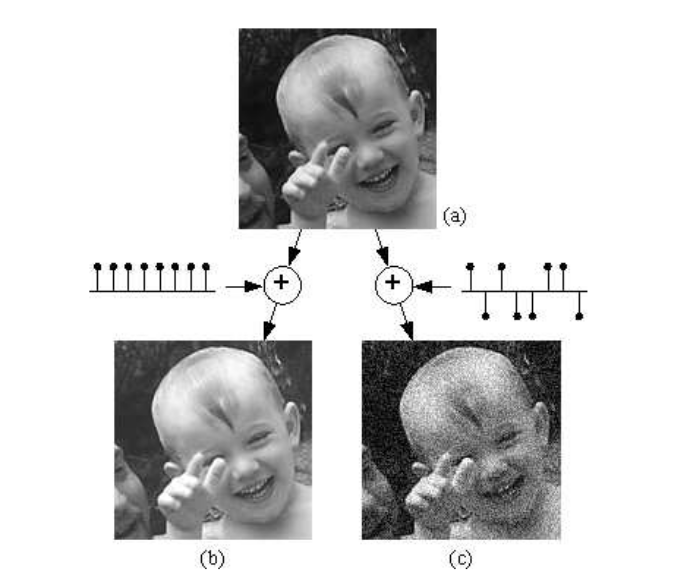
\includegraphics[width=0.6\textwidth]{imagenes/chapter2/failure_minkowski_metric.png}
  \end{center}
  \caption{En este ejemplo, extraído de\cite{MinkowskiFailure},
  vemos que sumar una constante positiva a una imagen  de referencia (a) produce la imagen (b) que contiene la misma distancia \emph{Minkowski}\footnotemark[2]
  que (c), imagen fabricada por la misma constante pero permutando signo de forma aleatoria. Siendo que
  la percepción final es que la imagen (c) es peor que la imagen (b).
\label{fig:FailureMinkowskiMetric}}
\end{figure}
\begin{figure}[htp]
  \begin{center}
    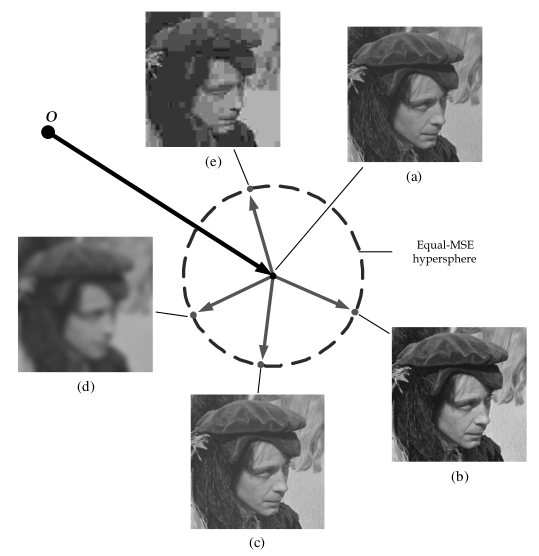
\includegraphics[width=0.6\textwidth]{imagenes/chapter2/MSE_Hypersphere.png}
  \end{center}
  \caption{En este ejemplo, extraído de\cite{Wang2006ModernIQ}, la misma imagen distorsionada de distintas maneras
  resulta en el mismo valor \emph{MSE}\footnotemark[3]=181. Siendo evidente que 
algunas distorsiones producen efectos visuales más marcados que otras.}
  \label{fig:MSEHyperSphere}
\end{figure}


\section{Aprendizaje Automático}
El aprendizaje automático\cite{IAModernApproach} o \emph{MachineLearning} (\emph{ML}) 
es una de las ramas que compone lo que definimos como 
la inteligencia artificial (\emph{IA}). Esta última se puede definir, 
según\cite{WhatIsAI}, como 
``La ciencia e ingeniería 
de crear máquinas inteligentes, especialmente programas de computadora inteligentes. 
Está relacionada con la tarea similar de utilizar computadoras para comprender 
la inteligencia humana...''

En este caso hablamos de dar soluciones a problemas complejos sin 
solución analítica (o que resulta muy costoso hallarla), es decir, necesitamos que la computadora sea la que identifique
los patrones en los datos y realice predicciones sobre ellos\cite{LearningFromData}.
Se puede definir más formalmente que un programa aprende de la experiencia E con
respecto a alguna clase de tareas T y una métrica de rendimiento P si su
rendimiento en las tareas T, medido con P, mejora con la experiencia E\cite{TomMitchell}.

Dependiendo de factores como las necesidades del problema, la naturaleza
de los datos a utilizar o el objetivo a alcanzar, podemos encontrar distintos tipos de
algoritmos de aprendizaje. En este documento se recogerán dos grandes grupos: aprendizaje supervisado 
y aprendizaje no supervisado. En el primero disponemos de un conjunto de datos 
anotados, es decir, con las salidas deseadas para cada ejemplo y en el segundo 
se espera que sea la máquina la que determine los patrones~(\ref{fig:SupervisedExample}, \ref{fig:UnsupervisedExample}). 

En general se suelen aplicar las técnicas de \emph{ML} sobre grandes conjuntos 
de datos sobre los cuales deseamos detectar los patrones subyacientes\cite{
DataMiningHandbook}.

Puede observarse que dada estas descripciones, al problema presente podemos 
aplicarle alguna técnica de \emph{ML}: Tenemos datos de entrada (caracteríticas 
extraídas de nubes de puntos distorisionadas) y una salida (valor de calidad). Además, existen conjuntos de 
datos públicos etiquetadas para distintos tipos de distorsiones. Esto significa que
estamos entre un problema de aprendizaje supervisado.

\begin{figure}[htp]
  \centering
    \begin{subfigure}{.3\textwidth}
  \centering
  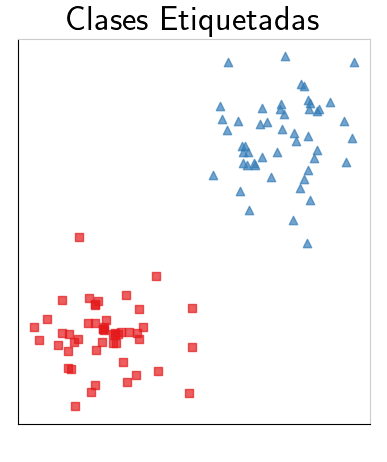
\includegraphics[width=0.8\linewidth]{imagenes/chapter2/BeforeSVMExample.png} 
  \tikz[remember picture]\node[inner sep=0pt,outer sep=0pt] (a) {}; 
    \end{subfigure}
    \begin{subfigure}{.3\textwidth} 
  \centering
  \tikz[remember picture]\node[inner sep=0pt,outer sep=0pt] (b) {}; 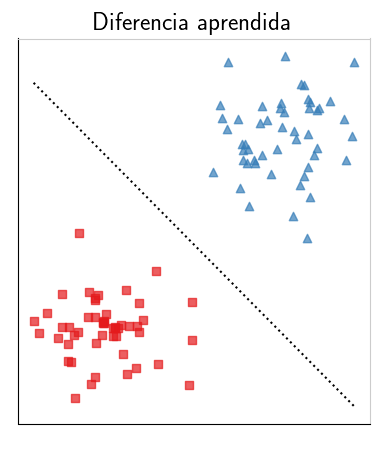
\includegraphics[width=0.8\linewidth]{imagenes/chapter2/AfterSVMExample.png}
    \end{subfigure}
  \tikz[remember picture,overlay]\draw[line width=1pt,-stealth,black] ([xshift=2mm,yshift=2cm]a.east) -- ([xshift=-2mm, yshift=2cm]b.west)node[midway,above,text=black,font=\LARGE\bfseries\sffamily] {};
  \caption{
  Ejemplo de aprendizaje supervisado, vemos como a partir de un conjunto de clases etiquetadas aprendemos un hiper plano que 
  las separa. 
  }
  \label{fig:SupervisedExample}
\end{figure}
\begin{figure}[htp]
  \centering
    \begin{subfigure}{.3\textwidth}
  \centering
  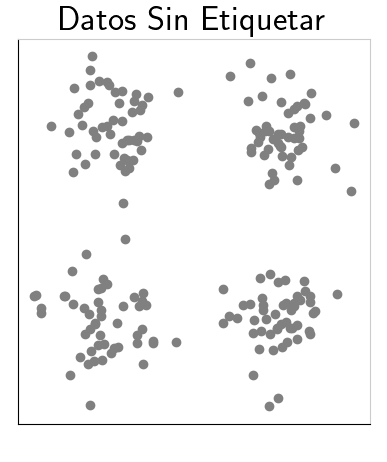
\includegraphics[width=0.8\linewidth]{imagenes/chapter2/BeforeClusteringExample.png} 
  \tikz[remember picture]\node[inner sep=0pt,outer sep=0pt] (c) {}; 
    \end{subfigure}
    \begin{subfigure}{.3\textwidth} 
  \centering
  \tikz[remember picture]\node[inner sep=0pt,outer sep=0pt] (d) {}; 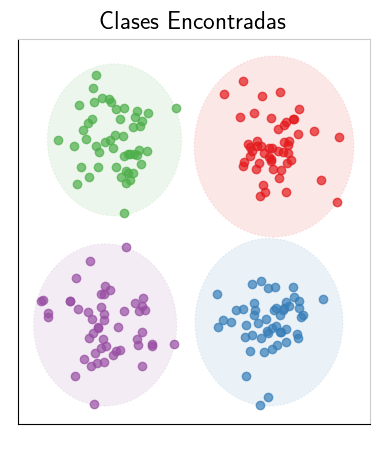
\includegraphics[width=0.8\linewidth]{imagenes/chapter2/AfterClusteringExample.png}
    \end{subfigure}
  \tikz[remember picture,overlay]\draw[line width=1pt,-stealth,black] ([xshift=2mm,yshift=2cm]c.east) -- ([xshift=-2mm, yshift=2cm]d.west)node[midway,above,text=black,font=\LARGE\bfseries\sffamily] {};

  \caption{
  Ejemplo de aprendizaje no supervisado, dado un conjunto de puntos aprendemos un conjunto de clases 
  a partir de los patrones.
}
  \label{fig:UnsupervisedExample}
\end{figure}

\section{Aprendizaje Profundo}
En el aprendizaje profundo o \emph{Deep Learning} (\emph{DL}), 
a diferencia de los modelos anteriores donde tenemos un conjunto de variables 
extraídas por un humano experto, las características sobre la cual inferimos 
son obtenidas por el propio modelo automáticamente\cite{DeepLMITPress, DeepLearningNature, DeepLearningInNN}.
En términos generales, la extracción automática de características suele 
desempeñar mejores resultados en contra de las características manuales.

La mayoría de los modelos de DL son basados en múltiples capas jerárquicas de 
procesado de datos. Las más conocidas son las redes neuronales (ANN, por sus siglas 
en inglés), modelo bioinspirado que simula el funcionamiento de las neuronas del cerebro
humano (abstracción simplificada)\cite{ANNForPattern,ANNCambridge}. 

A alto nivel, el funcionamiento de una red neuronal implica tres etapas principales: 
entrada, procesamiento y salida. En la etapa de entrada, se proporciona a la red 
neuronal un conjunto de datos o características que representan la información 
que se desea analizar o procesar. Estos datos de entrada se propagan a través 
de la red neuronal (\emph{feedforward}). En la etapa de procesamiento, las neuronas reciben las entradas 
y realizan cálculos utilizando pesos y funciones de activación. Los pesos representan 
la importancia relativa de las diferentes entradas en el cálculo, y las funciones 
de activación determinan la salida de una neurona en función de su entrada. A medida que los datos se propagan a través de la red neuronal, las capas intermedias 
procesan y combinan las entradas, extrayendo características relevantes y creando 
representaciones internas cada vez más abstractas. Esto permite que la red neuronal aprenda y 
descubra patrones en los datos. Finalmente, en la etapa de salida, la red neuronal 
produce una respuesta o predicción basada en las características extraídas. 
Esto puede ser la clasificación de una imagen, la predicción de un valor numérico o 
cualquier otro resultado deseado. En esta última etapa se calcula el error de 
predicción respecto a la salida deseada con la función de pérdida y se ajusta 
los pesos respectivamente.

El aprendizaje de una red neuronal se logra mediante un proceso llamado entrenamiento.
Donde de forma iterativa repetimos el proceso descrito anteriormente varias veces 
con distintos ejemplos. El conjunto de datos es muy relevante para el correcto 
aprendizaje. Debe de ser representativo, extenso y limpio de anormalidades ya que 
estaremos extrayendo características y relevancias a partir de ellos.

En definitiva, una red neuronal es en esencia una serie de ajustes de parámetros para lograr el resultado deseado. 
Estos incluyen ajuste de los pesos y sesgos iniciales, selección de las funciones de activación, 
como las más utilizadas sigmoide o ReLU, de una función de pérdida y un optimizador, 
encargado de determinar como ajustar los pesos según el error obtenido en cada fase del entrenamiento.
No obstante, existe un fenómeno denominado sobreentrenamiento o \emph{overfitting}. 
Ocurre cuando hay un sobreajuste de los parámetros
hacia los datos de entrenamiento, disminuyendo la capacidad de generalización del modelo. 
Informalmente, es como decir que el modelo ha memorizado los resultados y por ello 
con datos nunca vistos posee errores substancialmente altos. Para lidiar con estos 
problemas se deben eliger también formas de regularización del modelo, es decir, 
restricción sobre el entrenamiento para evitar el sobre ajuste. 

\begin{figure}[htp]
  \centering
  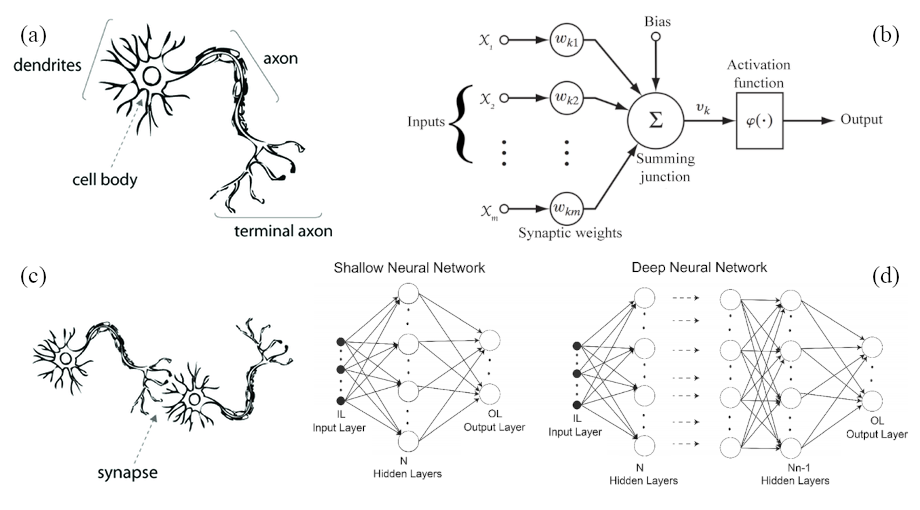
\includegraphics[width=\textwidth]{imagenes/chapter2/ANNVisualization.png}
  \caption{Ejemplo gráfico de una red neuronal\cite{
    NeuronImages, NeuronSimilarity, ShallowAndDeepNN
    }. En (a) vemos una neurona con 
  su representación artificial simplificada (b). En (c) vemos una conexión entre 
  neuronas y en (d) la representación de diferentes profundidades de conexiones artificiales}
  \label{fig:ANNVisualization}
\end{figure}

\subsection{Redes Convolucionales} 
Las redes convolucionales o \emph{convolutional neural network} (CNN)\cite{ConvolutionalZipCode, ConvolutionInRadiology}
son un tipo de arquitectura de redes neuronales diseñadas 
específicamente para el procesamiento de datos estructurados en forma de matrices, como imágenes.
Se ha descubierto que son aplicables para el procesado de texto, sonidos y, recientemente,
a superficies tridimensionales.
Utilizan capas convolucionales que aplican filtros a regiones locales de la entrada 
para extraer características relevantes. En la figura (\ref{fig:RadiographyConvolutionExample})
podemos ver un ejemplo de esquema jerárquico de extracción de características para el 
diagnóstico médico a partir de una radiografía. Con ese ejemplo se puede observar 
las diferencias con respecto a las ANN, posee dos capas adicionales: capas convolucionales 
y capas de \emph{pooling}.

\begin{figure}[htp]
  \centering
  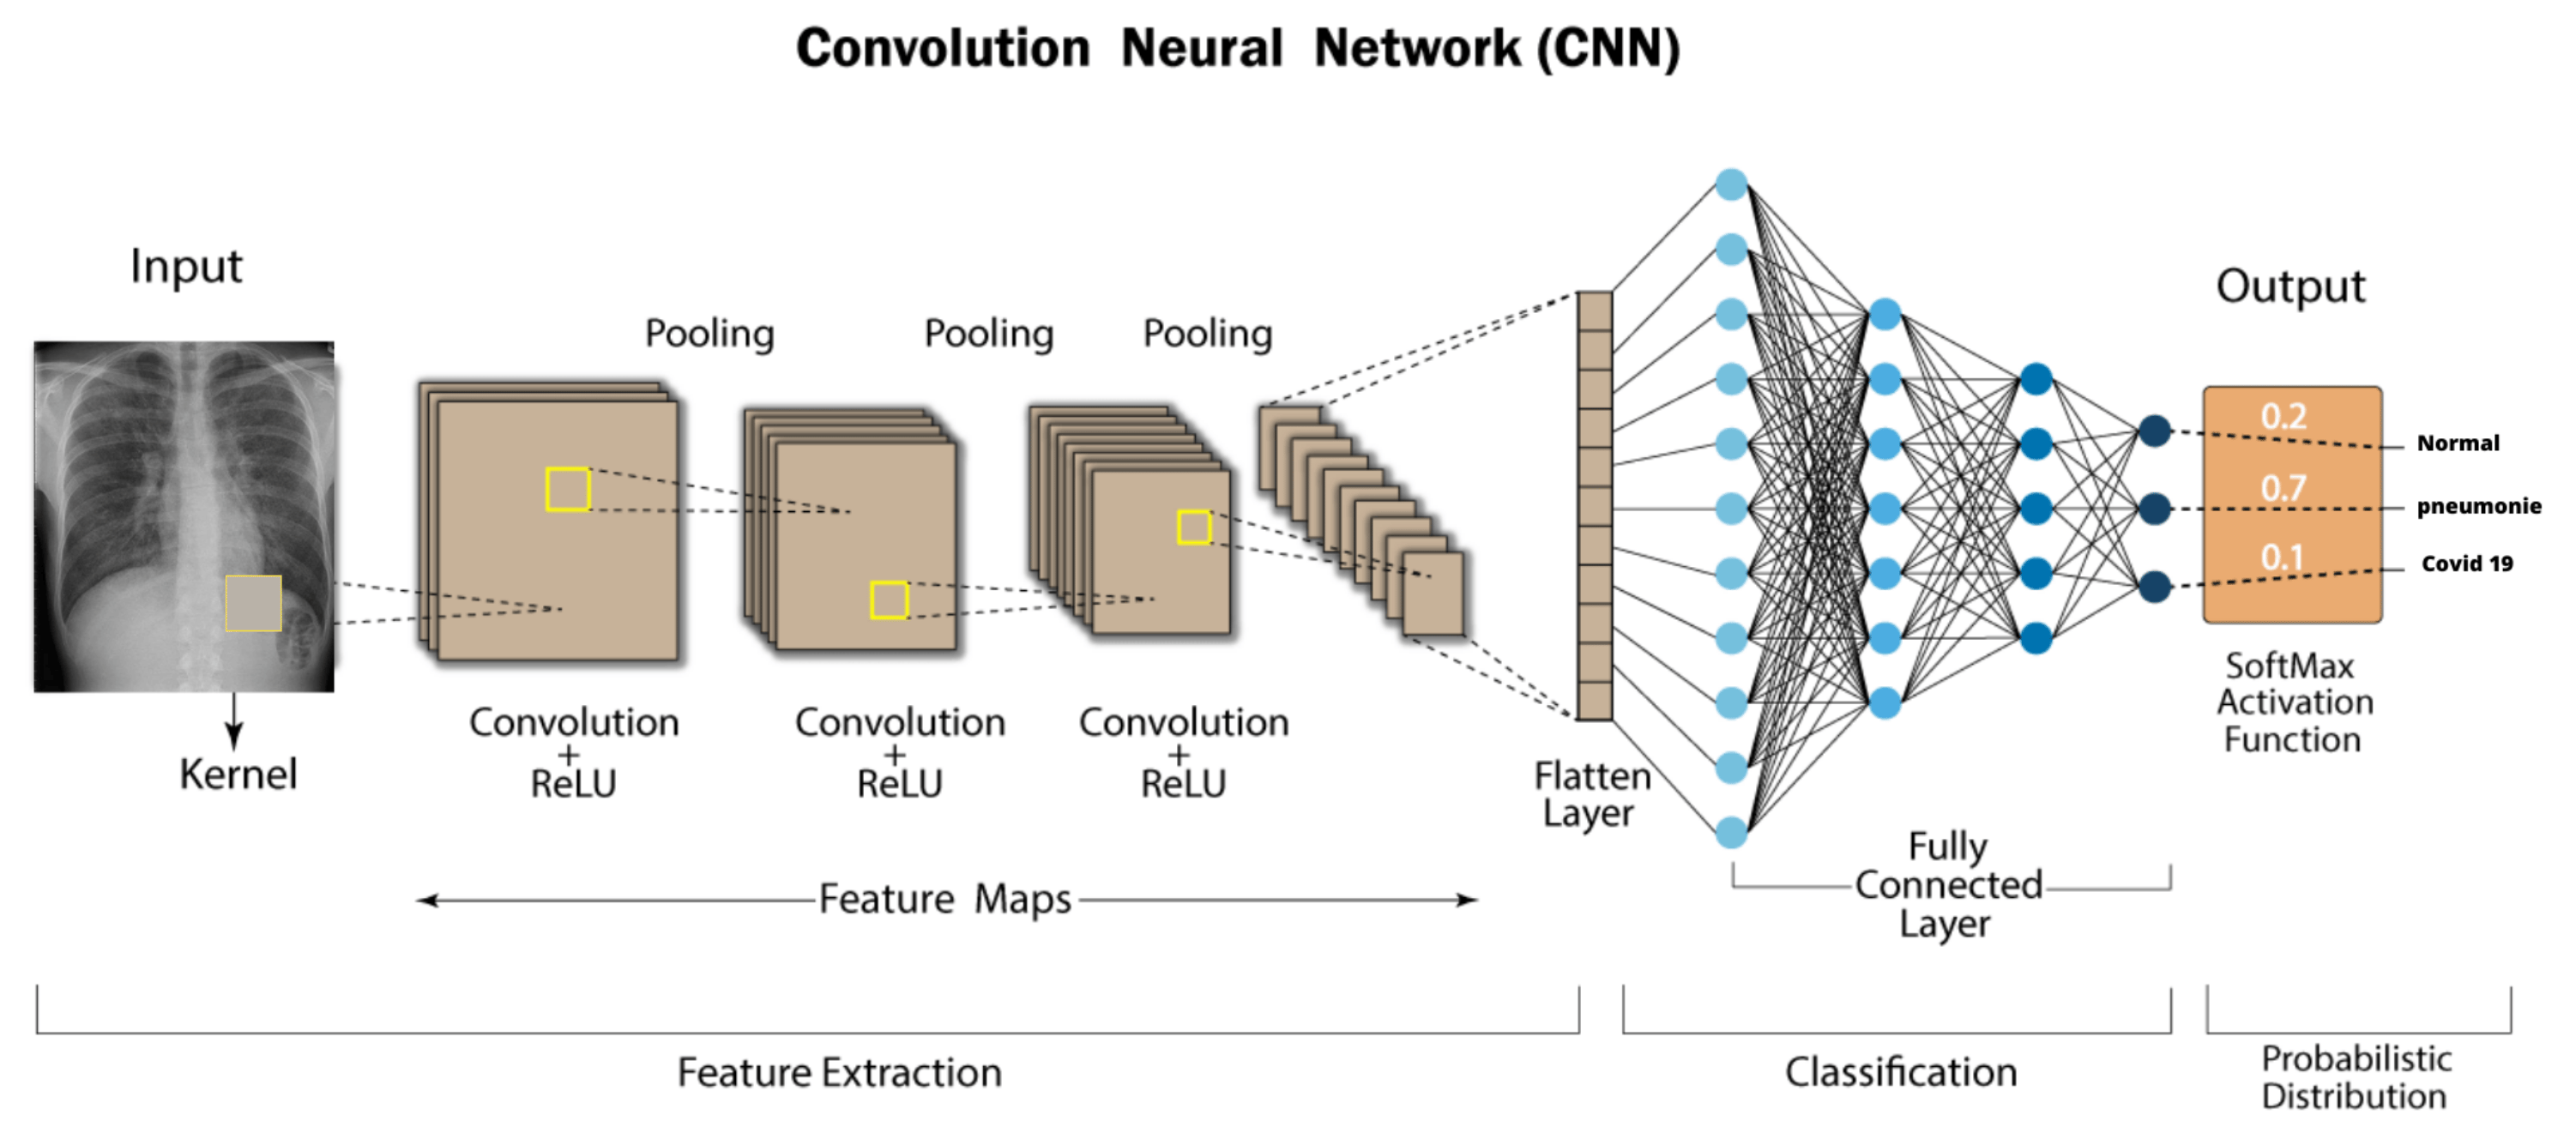
\includegraphics[width=\textwidth]{imagenes/chapter2/RadiographyConvolutionExample.png}
  \caption{Ejemplo extraída de \cite{RadiographyConvolutionExample} del proceso de convolución sobre una radiografía pulmonar 
  para la detección de enfermedades.}
  \label{fig:RadiographyConvolutionExample}
\end{figure}

\subsection{Capas convolucionales}
Para simplificar la explicación, la realizaremos sobre imágenes 2D. 
Una capa convolucional es encargada de realizar la operación de convolución sobre 
los datos de entrada. 
La convolución se refiere a una operación matemática que combina dos funciones para crear una tercera función.
En este caso, se aplica una operación de convolución 
entre una matriz de entrada (como una imagen) y un filtro (\emph{kernel}).
La operación de convolución implica deslizar el filtro sobre la matriz de entrada, 
multiplicando los elementos coincidentes y sumándolos para obtener un único valor 
en la matriz de salida, conocida como mapa de características. 
Este proceso se repite en diferentes ubicaciones de la matriz de 
entrada para generar el mapa de características completo. En la figura 
(\ref{fig:ConvolutionalRepresentation}) vemos una operación sobre la ubicación 
inicial de la imagen, esquina superior izquierda. 
La elección del siguiente trozo 
o \emph{patch} de la imagen suele venir determinado por el paso o \emph{stride}.
Habitualmente se utiliza un \emph{stride} de 1. Es decir, elegimos la matriz 
adyaciente con distance horizontal igual a 1 hasta llegar al final de esa fila 
y luego nos deplazamos 1 hacia abajo. 
Por medio de este proceso, la red es capaz de
capturar dependencias temporales y espaciales en los datos con la aplicación
de los filtros relevantes.

Podemos observar en (\ref{fig:ConvolutionalRepresentation} que aplicar directamente 
el operador de convolución a una imagen resulta en una reducción del tamaño del mapa 
de activación debido a la naturaleza del operador. 
Sin embargo, esto no siempre es deseable. 
Para abordar este problema, se puede agregar relleno o \emph{padding} a la imagen 
de entrada utilizando información existente en la misma. 
Esto garantiza que el mapa de activación tenga la misma dimensionalidad que 
la imagen original. Además, es posible reducir aún más la salida ajustando 
los saltos o \emph{strides} del filtro de convolución mientras se recorre la imagen.

\begin{figure}[htp]
  \begin{center}
    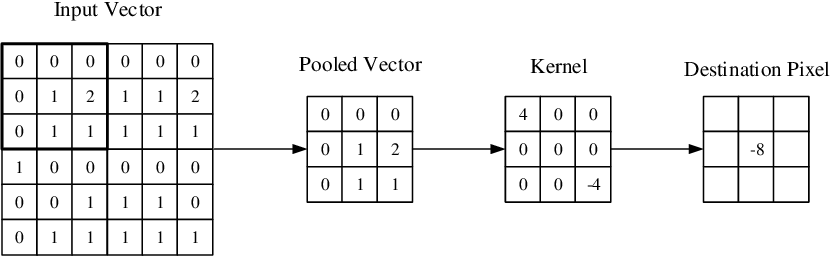
\includegraphics[width=0.95\textwidth]{imagenes/chapter2/ConvolutionalRepresentation.png}
  \end{center}
  \caption{Representación visual de la operación de convolución sobre una imagen, extraída de\cite{ConvolutionalRepresentation}.
  }
  \label{fig:ConvolutionalRepresentation}
\end{figure}

\subsection{Capa de pooling} 
El propósito principal de las capas de \emph{pooling} es reducir la cantidad de parámetros 
y la complejidad computacional de la red, al tiempo que conservan las características 
más relevantes. Además, el \emph{pooling} puede ayudar a hacer que la representación sea 
invariante a pequeñas variaciones en la posición o el tamaño de los objetos en la 
imagen, lo que mejora la capacidad de generalización del modelo.

En la figura (\ref{fig:PoolingExample}) vemos un operador de \emph{pooling} común,
el operador de valor máximo. También es habitual el uso del operador de valor medio y
valor mínimo.
El pooling, al igual que la convolución, posee un filtro o ventana que recorre
los datos dado un salto o stride al moverse por los mismos,

Las capas convolucionales y de pooling trabajan en conjunto para procesar y extraer 
características. 
Dependiendo de la complejidad del problema, se puede ajustar el número de estas.

\begin{figure}[htp]
  \begin{center}
    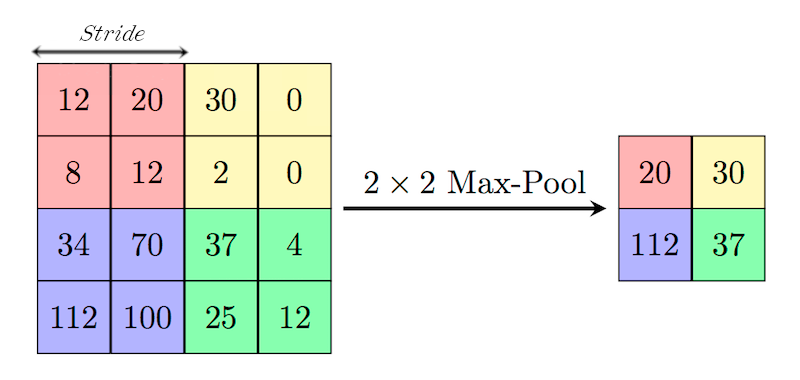
\includegraphics[width=0.65\textwidth]{imagenes/chapter2/MaxpoolSample.png}
  \end{center}

  \caption{
    Ejemplo de operación de \emph{max-pooling} con \emph{stride} a 2.
  }
  \label{fig:PoolingExample}
\end{figure}

\subsection{Capas totalmente conectadas}
Las capas totalmente conectadas o \emph{fully connected}, también llamadas 
capas densas o \emph{dense}, son aquellas en las que todas sus neuronas 
están conectadas con todas las neuronas de la capa anterior y de la
siguiente. Si bien existen modelos totalmente convolucionales, resulta común
que las CNN's incluyan capas totalmente conectadas al final de la arquitectura.
Estas capas forman una ANN clásica.
La salida de la última capa densa, siendo la salida de la red entera, es donde
se evaluará la función de pérdida elegida, y al igual que en una red neuronal
clásica.


\subsection{Aplicadas a Videos} 

\section{Ensemble o Conjunto \emph{Deep Learning}}

\section{Imágenes médicas, Métricas y Distorsiones}
\label{sec:Distorsiones}
